
\documentclass{article}
\usepackage{graphicx} % Required for inserting images
\usepackage{fancyhdr} % Required for header and footer configuration
\usepackage[a4paper, margin=2.5cm, left=1.5cm, right=1.5cm, bottom=4cm]{geometry} % Required for setting page margins
\usepackage[T1]{fontenc}
\usepackage[default,oldstyle,scale=1]{opensans} % Utilizzo del font Open Sans
\usepackage{lipsum}
\usepackage{makeidx}
\usepackage{booktabs}
\usepackage{tabularray}
\usepackage[colorlinks=true, linkcolor=black, urlcolor=blue, citecolor=blue]{hyperref}
\usepackage{tabularx}
\usepackage{makecell}
\usepackage{enumitem} % Pacchetto per la personalizzazione degli elenchi
\usepackage{booktabs}
\usepackage{subcaption}
\usepackage{pgfplots}
\usepackage{float}
\usepgfplotslibrary{dateplot} % Per gestire gli assi con date

% Configure header and footer for the first page
\fancypagestyle{firstpage}{
    \fancyhf{} % Clear header and footer
    \renewcommand{\headrulewidth}{0pt} % Remove header rule line
    \lhead{} % Header on the left
    \chead{} % Header in the center
    \rhead{} % Header on the right
    \lfoot{} % Footer on the left
    \cfoot{\vspace{5pt}\\\hrulefill\\\vspace{10pt}\textbf{BeeLive}\\Gruppo 21} % Footer in the center
    \rfoot{\vspace{32.5pt}\\\thepage} % Footer on the right
}

% Configure header and footer for non-plain pages (second page onwards)
\fancypagestyle{nonplain}{
    \fancyhf{} % Clear header and footer
    \lhead{} % Header on the left
    \chead{} % Header in the center
    \rhead{
\includegraphics[width=2cm]{Images/BeeLive-Logo.png}\\\vspace{2pt}} % Header on the right
    \lfoot{} % Footer on the left
    \cfoot{\vspace{5pt}\\\hrulefill\\\vspace{10pt}\textbf{BeeLive}\\Gruppo 21} % Footer in the center
    \rfoot{\vspace{32.5pt}\\\thepage} % Footer on the right
}

% Adjust vertical space between header and text                                    
\setlength{\headsep}{65pt} 
% Adjust vertical space between text and footer
\setlength{\footskip}{0pt} 

\title{
\includegraphics[width=0.75\textwidth]{Images/BeeLive-Logo.png}\\\vspace{100pt}
\LARGE{\textbf{BeeLive\\Deliverable 4}}}
\author{Gruppo 21:\\
Cipriani Pietro, 226959\\
Orlando Dennis, 227688\\
Ziviani Elia, 228172}
\date{11 Giugno 2024}

\makeindex % Indica che vogliamo creare un indice

\begin{document}

\maketitle
\thispagestyle{firstpage} % Apply firstpage style to the first page
\clearpage

\pagestyle{nonplain} % Apply non-plain style to subsequent pages

\renewcommand{\contentsname}{Indice}
\tableofcontents

\clearpage

\section{TODO}
\begin{itemize}
    \item Revisione generale del documento
    \item BurnDown chart
    \item TestCases - Revisione con test \texttt{public-server}
    \item Product backlog refinement
    \item Sprint retrospective
    \item Diagramma deploy finale
    \item Conclusioni
\end{itemize}

\clearpage

\section{Revisione}
...

\clearpage

\section{Introduzione}

\subsection{Componenti del gruppo}
\begin{itemize}
    \item Cipriani Pietro, matricola 226959, \lbrack\href{https://github.com/pietrocipriani}{github profile}\rbrack
    \item Orlando Dennis, matricola 227688, \lbrack\href{https://github.com/dennisorlando}{github profile}\rbrack
    \item Ziviani Elia, matricola 228172, \lbrack\href{https://github.com/ELI20ZIVI}{github profile}\rbrack
\end{itemize}

\subsection{Scopo del progetto}

Lo scopo del progetto 'BeeLive' è quello di risolvere il problema riguardante la difficoltà nel reperire informazioni riguardanti gli eventi che influenzano la viabilità all'interno del Comune di Trento. Prevediamo un sistema informativo, dedicato agli utenti cittadini, che mostri visualmente le variazioni della viabilità in città, informando gli stessi di eventuali modifiche che potrebbero colpirli direttamente.

\subsection{Link utili}
Il primo link fornito è quello della repository github. La repository è stata creata appena il corso è cominciato, infatti inizialmente è risultata utile al fine di scrivere in modo collaborativo i primi deliverable.\\
E' stato deciso di integrare in questa repository anche le fasi di sprint in quanto come team riteniamo utile la possibilità di accedere alla documentazione redatta nei primi due deliverable.\\
La repository è accessibile al seguente link: \href{https://github.com/ELI20ZIVI/BeeLive/}{Repository GitHub}\\ \\
Il secondo link fornito è quello di Apiary. Apiary è uno strumento che permette di creare e documentare in modo molto accurato e approfontido le API utilizzate nel progetto.\\
Il link di Apiary è il seguente: \href{https://beelive.docs.apiary.io/#}{Link Apiary}\\ \\
Per eseguire un deploy del progetto sarà necessario installare i due applicativi (Mobile e Desktop). Il link per scaricarli e testarli è \href{github-release-page}.\\
Gli account da utilizzare per il login all'applicativo desktop sono i seguenti:
\begin{itemize}
    \item Utente Autorizzato: Username: \textit{user1}, Password: \textit{password1}
    \item Utente Amministratore: Username: \textit{user2}, Password: \textit{password2}
\end{itemize}
L'utilizzo dell'applicativo mobile non richiede un login, in quanto, siccome le funzionalità di un utente autenticato e un utente non sono le stesse, come gruppo abbiamo deciso di focalizzarci su altre funzionalità che abbiamo ritenuto più importanti.

\clearpage

\section{Sezione generale}

\subsection{Strategia di Branching}
Anche per questo secondo sprint è stata evitata la strategia di branching "Master only", infatti come descritto nel documento "Deliverable 3", per noi la creazione e l'utilizzo di un unico branch principale \textit{main} avrebbe causato problemi di collaborazione e conflitti nel momento in cui tutti i componenti sarebbero andati a lavorare conteporaneamente a stesse sezioni del progetto. \\

\noindent
Abbiamo quindi deciso di mantenere la stessa metodologia di branching dello scorso sprint, ossia la \textit{Feature Branching} con però un branch \texttt{develop}, precedente al branch \texttt{main}, sul quale, una volta ritenute soddisfacenti le modifiche e le feature aggiunte, queste vengono integrate.\\
Quando le features sono tutte integrate nel branch \texttt{develop}, questo viene, una volta che tutto è testato nei minimi dettagli, integrato nel branch \texttt{main} come operazione di 'release'.\\

\noindent
Tramite questo approccio puntiamo ad incrementare la collaborazione tra i membri del team, ridurre i conflitti e le inconsistenze nel codice, facilitare la gestione delle diverse attività in corso e mantenere inoltre una mappatura di tutte le diverse modifiche e progressi del progetto, mantenendo ben strutturata la storia del codice.\\

Segue una lista dei branch utilizzati per lo sviluppo del progetto; da notare che molte di queste branches sono state eliminate una volta integrate in \texttt{develop}, per cui su github potrebbero non apparire.

\subsubsection{\texttt{main}}

Il branch principale del progetto, in cui vengono integrate tutte le funzionalità completate e testate.\\
Tutte le funzionalità all'interno di questo branch sono considerate terminate e funzionanti, pronte per essere rilasciate.

\subsubsection{\texttt{develop}}

Il branch di sviluppo del progetto, in cui vengono integrate tutte le funzionalità completate e testate.\\
Non e' pensato propriamente come il branch in cui vengono rilasciate le funzionalita' ma piuttosto come un branch di supporto per il branch principale, infatti in questo branch vengono prima caricate le funzionalita' dagli altri branch specifici e successivamente testate.\\
Una volta che sono considerate funzionanti sono quindi integrate nel branch principale.

\subsubsection{\texttt{preview}}

Branch dedicato alla preview dell'interfaccia grafica dei due applicativi.\\
E' stato utilizzato al momento della prima presentazione del progetto per mostrare il lavoro svolto ai committenti e per ricevere feedback su eventuali modifiche da apportare.\\
Integra dei mockup delle varie interfacce, desktop e mobile, che andranno sviluppate.\\
Parte della preview relativa all'applicativo desktop è stata poi utilizzata in \texttt{da\_frontend} come punto di partenza per l'interfaccia.

\subsubsection{\texttt{deliverable}}

Branch dedicato alla stesura dei vari documenti di deliverable.\\
Creato per mantenere separata la stesura della documentazione dal codice sorgente e per rispettare la metodologia di branching.

\subsubsection{\texttt{refactoring}}

Questo branch nasce per la necessità di effettuare refactoring sul codice prodotto. Prima di eseguire il merge in \texttt{main} spesso risulta necessario effettuare delle modifiche al codice per renderlo più leggibile, mantenibile e performante.\\
Avendo un ambiente separato si annulla la possibilità di introdurre errori nel codice principale.

\subsubsection{\texttt{deployment}}

Branch dedicato alla preparazione del deploy del progetto.\\
Vengono preparate tutte le componenti alla fase di deploy, come la creazione dei file di configurazione, la preparazione dei file per il deploy e la creazione di script per automatizzare il deploy.

\subsubsection{\texttt{management-server}}

Branch dedicato allo sviluppo del server di gestione, il server utilizzato dall'applicativo desktop (Quindi dagli utenti autorizzati) per eseguire tutte le operazioni di gestione degli eventi.

\subsubsection{\texttt{public\_server}}

Similmente al branch precedente, questo branch è dedicato allo sviluppo del server pubblico, il server utilizzato dall'applicativo mobile (Quindi dagli utenti comuni) per la visualizzazione degli eventi e le varie impostazioni dell'applicativo.

\subsubsection{\texttt{da\_frontend}}

Branch dedicato allo sviluppo dell'interfaccia grafica dell'applicativo desktop.\\
In questo branch vengono sviluppate tutte le componenti che caratterizzano l'interfaccia grafica dell'applicativo desktop.

\subsubsection{\texttt{da\_authn}}

Il branch è dedicato allo sviluppo del modulo di autenticazione dell'applicativo desktop.\\
Include infatti tutto il codice e la logica necessari all'autenticazione degli utenti autorizzati e dell'utente amministratore all'applicativo desktop.

\subsubsection{\texttt{da\_event\_list}}

Branch di sviluppo della funzionalità di visualizzazione a lista degli eventi a disposizione dell'utente che ha eseguito il login all'applicativo desktop.\\
E' integrata tutta la logica di richiesta delle informazioni al server e di visualizzazione delle stesse in modo chiaro e ordinato.

\subsubsection{\texttt{ma\_client}}

Branch dedicato allo sviluppo del client mobile, i.e. l'applicazione mobile utilizzata dagli utenti comuni (autenticati e non) che intendono visualizzazione le criticita' presenti in citta'.\\
Il branch, una volta concluso lo sviluppo dell'applicativo, e' stato integrato nel branch \texttt{develop} per i test in associata con tutti gli altri moduli.


\subsubsection{\texttt{ma\_screen}}

Branch dedicato alla creazione delle schermate dell'applicativo mobile, i.e. tutte le schermate che l'utente visualizzera' durante l'utilizzo dell'applicativo.\\
Questo branch è stato integrato in \texttt{ma\_client} in quanto sua dipendenza.

\subsubsection{\texttt{ma\_details}}

Il branch nasce con lo scopo di mantenere il codice dell'interfaccia di visualizzazione degli eventi e dei rispettivi sottoeventi sull'applicativo mobile.
Branch successivamente integrato in \texttt{ma\_client} in quanto sua dipendenza.

\subsubsection{\texttt{ma\_map}}

Branch utilizzato per sviluppare la libreria che permette di integrare la mappa interattiva all'interno dell'applicativo mobile.\\
Questa libreria permette di visualizzare in modo chiaro e intuitivo le criticita' presenti in citta' e di visualizzare la posizione degli eventi.

\subsubsection{\texttt{ws-fetch-event}}

Branch dedicato allo sviluppo del webserver pubblico, i.e. il webserver in cui sono stati implementati gli endpoint API dedicati al fetching di eventi ad opera dell'applicativo mobile.\\
Una volta che il modulo e' stato completato, e' stato integrato nel branch \texttt{develop} per i test con tutti gli altri moduli.

\subsubsection{\texttt{ws-insert-event}}

Branch dedicato allo sviluppo del webserver gestionale, i.e. il webserver in cui sono stati implementati gli endpoint API dedicati all'inserimento degli eventi all'interno del sistema ad opera dell'applicativo desktop. \\
Utile allo sviluppo del modulo utilizzato dall'applicativo desktop per l'inserimento delle criticita' in citta'.
Una volta che il modulo e' stato completato, e' stato integrato nel branch \texttt{develop} per i test con tutti gli altri moduli.\\
Delle versioni intermedie di questa branch sono state usate da altre branches, in particolare da \texttt{da\_desktop}, in quanto necessaria per effettuare il testing di quest'ultima.

\clearpage

\subsection{Product Backlog}
Nella pagina seguente vi è riportato il product backlog che abbiamo sviluppato per questo progetto. E' possibile notare una linea di demarcazione che limita inferiormente le entries selezionate per il primo sprint.

\begin{table}[!ht]
    \centering
    \renewcommand{\arraystretch}{1.3} % Imposta lo spazio verticale delle righe
    \begin{tabularx}{\textwidth}{| r | X | r | r |}
        \Xhline{2pt}
        \makecell{\textbf{Nome}} & \makecell{\textbf{User story}} & \makecell{\textbf{Priorità}} & \makecell{\textbf{Stima}} \\
        \Xhline{2pt}
        \makecell{Accesso alle\\criticità} & \makecell{Da utente, voglio essere in grado di visualizzare la lista\\degli eventi che ci sono in città} & \makecell{200} & \makecell{8}\\
        \hline
        \makecell{Accesso al\\programma\\desktop} & \makecell{\textbf{NUOVO} Da utente autorizzato, voglio essere in grado di accedere\\all'applicativo desktop in modo da poter operare\\sulle criticità a me associate} & \makecell{190} & \makecell{8}\\
        \hline
        \makecell{Aggiunta eventi\\da utente\\autorizzato} & \makecell{Da utente autorizzato, devo essere in grado di aggiungere degli eventi\\in modo da comunicare la loro presenza agli utenti} & \makecell{180} & \makecell{8}\\
        \hline
        \makecell{Registrazione e\\accesso all'\\app mobile} & \makecell{Da utente, voglio essere in grado di poter registrare un account\\in modo da poter salvare le mie impostazioni\\e le aree di interesse che ho impostato} & \makecell{170} & \makecell{8}\\
        \hline
        \makecell{Visualizzazione\\criticità\\su mappa} & \makecell{Da utente, voglio visualizzare su una cartina le zone colpite dai diversi\\eventi, in modo da capire visivamente se in una zona che mi\\interessa vi è un evento attivo} & \makecell{160} & \makecell{6}\\
        \hline
        \makecell{Visualizzazione\\dei dettagli del\\singolo evento} & \makecell{Da utente, voglio avere } & \makecell{150} & \makecell{6}\\
        \Xhline{2pt}
        \makecell{Impostazione\\categorie\\d'interesse\\per gli eventi} & \makecell{Da utente, voglio essere in grado di impostare le categorie di eventi\\alle quali io sono interessato, in modo che la lista di eventi visibile\\dall'applicazione contenga solamente gli eventi che mi interessano,\\e in modo che io non venga notificato di alcun evento\\che io non ritenga appartenere ad una categoria interessante} & \makecell{100} & \makecell{5}\\
        \hline
        \makecell{Impostazione\\zone\\d'interesse} & \makecell{Da utente, voglio essere in grado di impostare delle zone di interesse,\\in modo che io venga notificato di qualsiasi evento che insorga\\in una di queste zone} & \makecell{90} & \makecell{7}\\
        \hline
        \makecell{Visualizzazione\\eventi\\di competenza} & \makecell{Da utente autorizzato, devo essere in grado di visualizzare gli eventi\\di mia competenza, in modo da sapere quali eventi sono stati creati e\\monitorare il loro stato} & \makecell{80} & \makecell{5}\\
        \hline
        \makecell{Modifica\\eventi} & \makecell{Da utente autorizzato, devo essere in grado di modificare degli eventi\\in modo da evitare errori comunicativi} & \makecell{75} & \makecell{2}\\
        \hline
        \makecell{Eliminazione\\eventi} & \makecell{Da utente autorizzato, devo essere in grado di eliminare degli eventi} & \makecell{40} & \makecell{2}\\
        \hline
        \makecell{Accesso\\account\\utente} & \makecell{Da utente registrato, voglio essere in grado di poter accedere al\\mio account in modo da poter riottenere le aree di interesse e\\le impostazioni che ho precedentemente salvato} & \makecell{70} & \makecell{3}\\
        \hline
        \makecell{Visualizzazione\\eventi\\di categorie\\di interesse} & \makecell{Da utente, voglio essere in grado di visualizzare solo\\eventi di categorie di interesse} & \makecell{60} & \makecell{3}\\
        \hline
        \makecell{Selezione\\percorso} & \makecell{Da utente, voglio essere in grado di selezionare un percorso a partire\\da dei waypoint, per impostare dei percorsi di interesse} & \makecell{40} & \makecell{2}\\
        \hline
    \end{tabularx}
    \caption{Product backlog}
\end{table}

\clearpage

\subsection{Definition of "Done"}
La seguente 'Definition of Done' è basata su una valutazione collettiva che ha preso in considerazione  diversi fattori riguardanti la qualità del lavoro, non ignorando però la fattibilità e la realizzabilità di questi.\\
I criteri inclusi nella nostra 'Definition of Done' definita per il progetto sono i seguenti:
\begin{itemize}
	\item \textbf{Funzionalità}: le funzionalità che il codice implementa devono soddisfare appieno l'usecase / gli usecase associati al codice.
    \item \textbf{Codice}: Il codice deve essere revisionato e la sua correttezza / adeguatezza approvata da almeno un altro membro del team.
    \item \textbf{Test}: Il codice deve essere adeguatamente coperto da test unitari, di integrazione e funzionali, che devono essere scritti e superati con successo. Un adeguato numero di questi test deve essere scritto da membri diversi.
    \item \textbf{Documentazione}: Il codice e le funzionalità implementate devono essere adeguatamente documentati. Questo giudizio di adeguatezza deve essere dato da almeno un altro membro del team.
    \item \textbf{Build e Deployment}: Il codice deve integrarsi con successo nella build principale e la sua inclusione nella build principale non deve assolutamente far fallire dei test, nel caso in cui quest'ultimi venivano correttamente superati priva dell'inclusione.
    \item \textbf{Performance}: le funzionalità e il codice introdotti non devono causare visibili degradi alle performance di nessun elemento del progetto.
    \item \textbf{Conformità}: Il prodotto deve essere conforme alle normative legali e agli standard di sicurezza e qualità specifici del settore.
\end{itemize}

\clearpage

\section{Sezione Sprint \#2}

\subsection{Goal dello sprint}

Per questo secondo sprint ci siamo dedicati a rifinire le funzionalità implementate nello sprint precedente.\\
Le funzionalità implementate fino a questo punto sono quelle che possiamo definire \textit{core}, ovvero quelle che sono essenziali per il funzionamento del progetto.\\
E' doveroso però specificare il fatto che, essendo il progetto in una fase iniziale, molte delle funzionalità implementate sono state sviluppate in modo molto basilare magari non includendo controlli e/o funzionalità che sarebbero state necessarie in un contesto reale.\\
Per questo motivo, in questo sprint ci siamo prefissati di migliorare e rifinire le funzionalità già implementate, aggiungendo controlli e funzionalità che riteniamo necessarie per un corretto funzionamento del progetto.\\

Inoltre in questo sprint saranno integrate anche nuove funzionalità, come la modifica e l'eliminazione degli eventi da parte dell'utente autorizzato tramite l'applicativo desktop, su cui ora è funzionante la gestione degli accessi per la verfica effettiva dell'utente.\\

\subsection{Sprint Planning}
Seguono le varie tabelle che riportano i task che ci siamo prefissati di portare a termine durante il secondo sprint.\\
Abbiamo preferito descrivere i task invece delle user stories in quanto per singola user story vi erano svariati sotto task da completare.\\
In questo modo i task sono stati divisi in modo più chiaro e preciso, permettendo una migliore gestione del lavoro, una maggiore chiarezza sulle attività da svolgere e una più grande possibilità di descrizione.\\

\subsubsection{Accesso alle criticità e ai loro dettagli}
Attività che riguardano la visualizzazione delle criticità presenti in città e dei dettagli di ciascuna di esse.\\
Include inoltre la ricostituzione di parti del progetto sviluppate durante il primo sprint che abbiamo deciso di correggere e migliorare.
\begin{table}[H]
    \centering
    \renewcommand{\arraystretch}{1.3} % Imposta lo spazio verticale delle righe
    \begin{tabularx}{\textwidth}{| X | r | r | r | r |}
        \Xhline{2pt}
        \makecell{\textbf{Nome}} & \makecell{\textbf{User story}} & \makecell{\textbf{Cosa fare}} & \makecell{\textbf{Assegnazione}} & \makecell{\textbf{Stima}} \\
        \Xhline{2pt}
        \makecell{1.\\Sistemazione\\codici di errore\\del public server} & \makecell{Da utente, voglio\\visualizzare la lista\\degli eventi in città} & \makecell{Nello sprint precedente erano\\stati definiti in modo poco chiaro\\alcuni codici di errore, che quindi\\vanno ridefiniti} & \makecell{Elia Ziviani} & \makecell{} \\
        \hline
        \makecell{2.\\Creazione\\dei test} & \makecell{Da utente, voglio\\visualizzare la lista\\degli eventi in città} & \makecell{Creazione dei test sulla\\base dei nuoi codici di\\errore per verificare l'effettivo\\funzionamento del componente} & \makecell{Elia Ziviani} & \makecell{} \\
        \hline
    \end{tabularx}
\end{table}
\vspace{-0.7cm}
\begin{table}[H]
    \centering
    \begin{tabularx}{\textwidth}{| X | r | r | r | r | r | r | r | r | r | r | r | r | r | r |}
        \Xhline{2pt}
        \textbf{No.} & \textbf{17/5} & \textbf{18/5} & \textbf{19/5} & \textbf{20/5} & \textbf{21/5} & \textbf{22/5} & \textbf{23/5} & \textbf{24/5} & \textbf{25/5} & \textbf{26/5} & \textbf{27/5} & \textbf{28/5} & \textbf{29/5} \\
        \Xhline{2pt}
        1. & 1 & 2 & 3 & 4 & 5 & 6 & 7 & 8 & 9 & 10 & 11 & 12 & 13 \\
        \hline
        2. & 14 & 15 & 16 & 17 & 18 & 19 & 20 & 21 & 22 & 23 & 24 & 25 & 26 \\
        \Xhline{2pt}
        \textbf{No.} & \textbf{30/5} & \textbf{31/5} & \textbf{ 1/6} & \textbf{ 2/6} & \textbf{ 3/6} & \textbf{ 4/6} & \textbf{ 5/6} & \textbf{ 6/6} & \textbf{ 7/6} & \textbf{ 8/6} & \textbf{ 9/6} & \textbf{10/6} & \textbf{11/6} \\
        \Xhline{2pt}
        1. & 1 & 2 & 3 & 4 & 5 & 6 & 7 & 8 & 9 & 10 & 11 & 12 & 13 \\
        \hline
        2. & 14 & 15 & 16 & 17 & 18 & 19 & 20 & 21 & 22 & 23 & 24 & 25 & 26 \\
        \hline
    \end{tabularx}
\end{table}

\clearpage

\subsubsection{Gestione degli eventi sul programma desktop}
Attività che riguardano la gestione degli eventi da parte dell'utente autorizzato tramite l'applicativo desktop.\\
Sono incluse anche in questo caso operazioni di ridefinizione di parti del codice sviluppato nel primo sprint che abbiamo deciso di correggere e migliorare.
\begin{table}[H]
    \centering
    \renewcommand{\arraystretch}{1.3} % Imposta lo spazio verticale delle righe
    \begin{tabularx}{\textwidth}{| X | r | r | r | r |}
        \Xhline{2pt}
        \makecell{\textbf{Nome}} & \makecell{\textbf{User story}} & \makecell{\textbf{Cosa fare}} & \makecell{\textbf{Assegnazione}} & \makecell{\textbf{Stima}} \\
        \Xhline{2pt}
        \makecell{1.\\Autogenerazione\\IDs} & \makecell{} & \makecell{Creazione del\\sottocomponente che\\si occupa di\\autogenerare gli ID} & \makecell{Dennis Orlando} & \makecell{} \\
        \hline
        \makecell{2.\\Sistemazione\\codici di errore\\(Management Server)} & \makecell{Da utente autorizzato,\\devo essere in grado\\di eliminare/modificare/\\creare degli eventi} & \makecell{Nello sprint precedente\\erano stati definiti\\in modo poco chiaro\\alcuni codici di errore,\\che quindi vanno ridefiniti} & \makecell{Dennis Orlando} & \makecell{} \\
        \hline
        \makecell{3.\\Restituzione\\nuovo ID} & \makecell{} & \makecell{Creazione del\\sottocomponente che\\si occupa di restituire\\l'ID} & \makecell{Dennis Orlando} & \makecell{} \\
        \hline
        \makecell{4.\\Redirecting alla\\pagina degli eventi\\dopo il publish} & \makecell{Da utente autorizzato,\\devo essere in grado di\\aggiungere degli eventi\\in modo da comunicare la\\loro presenza agli utenti} & \makecell{Creazione logica di\\redirecting alla pagina\\degli eventi dopo la\\creazione di un evento} & \makecell{Dennis Orlando} & \makecell{} \\
        \hline
        \makecell{5.\\No empty\\multipolygon when\\processing an Event\\with no SubEvents\\with polygons} & \makecell{Da utente autorizzato,\\devo essere in grado di\\aggiungere degli eventi\\in modo da comunicare la\\loro presenza agli utenti} & \makecell{...} & \makecell{Dennis Orlando} & \makecell{} \\
        \hline
    \end{tabularx}
\end{table}
\vspace{-0.7cm}
\begin{table}[H]
    \centering
    \begin{tabularx}{\textwidth}{| X | r | r | r | r | r | r | r | r | r | r | r | r | r | r |}
        \Xhline{2pt}
        \textbf{No.} & \textbf{17/5} & \textbf{18/5} & \textbf{19/5} & \textbf{20/5} & \textbf{21/5} & \textbf{22/5} & \textbf{23/5} & \textbf{24/5} & \textbf{25/5} & \textbf{26/5} & \textbf{27/5} & \textbf{28/5} & \textbf{29/5} \\
        \Xhline{2pt}
        1. & 1 & 2 & 3 & 4 & 5 & 6 & 7 & 8 & 9 & 10 & 11 & 12 & 13 \\
        \hline
        2. & 14 & 15 & 16 & 17 & 18 & 19 & 20 & 21 & 22 & 23 & 24 & 25 & 26 \\
        \hline
        3. & 27 & 28 & 29 & 30 & 31 & 32 & 33 & 34 & 35 & 36 & 37 & 38 & 39 \\
        \hline
        4. & 40 & 41 & 42 & 43 & 44 & 45 & 46 & 47 & 48 & 49 & 50 & 51 & 52 \\
        \hline
        5. & 53 & 54 & 55 & 56 & 57 & 58 & 59 & 60 & 61 & 62 & 63 & 64 & 65 \\
        \Xhline{2pt}
        \textbf{No.} & \textbf{30/5} & \textbf{31/5} & \textbf{ 1/6} & \textbf{ 2/6} & \textbf{ 3/6} & \textbf{ 4/6} & \textbf{ 5/6} & \textbf{ 6/6} & \textbf{ 7/6} & \textbf{ 8/6} & \textbf{ 9/6} & \textbf{10/6} & \textbf{11/6} \\
        \Xhline{2pt}
        1. & 1 & 2 & 3 & 4 & 5 & 6 & 7 & 8 & 9 & 10 & 11 & 12 & 13 \\
        \hline
        2. & 14 & 15 & 16 & 17 & 18 & 19 & 20 & 21 & 22 & 23 & 24 & 25 & 26 \\
        \hline
        3. & 27 & 28 & 29 & 30 & 31 & 32 & 33 & 34 & 35 & 36 & 37 & 38 & 39 \\
        \hline
        4. & 40 & 41 & 42 & 43 & 44 & 45 & 46 & 47 & 48 & 49 & 50 & 51 & 52 \\
        \hline
        5. & 53 & 54 & 55 & 56 & 57 & 58 & 59 & 60 & 61 & 62 & 63 & 64 & 65 \\
        \hline
    \end{tabularx}
\end{table}
\clearpage
\subsubsection{Accesso utente all'applicativo desktop}
Tutti i task che riguardano lo sviluppo dell'accesso all'applicativo desktop da parte dell'utente autorizzato.\\
\vspace{-0.3cm}
\begin{table}[H]
    \centering
    \renewcommand{\arraystretch}{1.3} % Imposta lo spazio verticale delle righe
    \begin{tabularx}{\textwidth}{| X | r | r | r | r |}
        \Xhline{2pt}
        \makecell{\textbf{Nome}} & \makecell{\textbf{User story}} & \makecell{\textbf{Cosa fare}} & \makecell{\textbf{Assegnazione}} & \makecell{\textbf{Stima}} \\
        \Xhline{2pt}
        \makecell{1.\\Token\\validation} & \makecell{Da utente autorizzato,\\voglio essere in grado di\\accedere all'applicativo desktop\\in modo da poter operare\\sulle criticità a me associate} & \makecell{Creazione della logica di\\validazione del toke ricevuto} & \makecell{Pietro Cipriani} & \makecell{} \\
        \hline
        \makecell{2.\\User info} & \makecell{} & \makecell{} & \makecell{} & \makecell{} \\
        \hline
    \end{tabularx}
\end{table}
\vspace{-0.7cm}
\begin{table}[H]
    \centering
    \begin{tabularx}{\textwidth}{| X | r | r | r | r | r | r | r | r | r | r | r | r | r | r |}
        \Xhline{2pt}
        \textbf{No.} & \textbf{17/5} & \textbf{18/5} & \textbf{19/5} & \textbf{20/5} & \textbf{21/5} & \textbf{22/5} & \textbf{23/5} & \textbf{24/5} & \textbf{25/5} & \textbf{26/5} & \textbf{27/5} & \textbf{28/5} & \textbf{29/5} \\
        \Xhline{2pt}
        1. & 1 & 2 & 3 & 4 & 5 & 6 & 7 & 8 & 9 & 10 & 11 & 12 & 13 \\
        \hline
        2. & 14 & 15 & 16 & 17 & 18 & 19 & 20 & 21 & 22 & 23 & 24 & 25 & 26 \\
        \Xhline{2pt}
        \textbf{No.} & \textbf{30/5} & \textbf{31/5} & \textbf{ 1/6} & \textbf{ 2/6} & \textbf{ 3/6} & \textbf{ 4/6} & \textbf{ 5/6} & \textbf{ 6/6} & \textbf{ 7/6} & \textbf{ 8/6} & \textbf{ 9/6} & \textbf{10/6} & \textbf{11/6} \\
        \Xhline{2pt}
        1. & 1 & 2 & 3 & 4 & 5 & 6 & 7 & 8 & 9 & 10 & 11 & 12 & 13 \\
        \hline
        2. & 14 & 15 & 16 & 17 & 18 & 19 & 20 & 21 & 22 & 23 & 24 & 25 & 26 \\
        \hline
    \end{tabularx}
\end{table}
\vspace{0.5cm}
\subsubsection{Ridefinizione e miglioramento del codice relativo all'applicativo mobile}
Tutte le modifiche di ridefinizione e miglioramento necessarie a rendere il codice dell'applicativo mobile migliore e più funzionale.\\
\vspace{-0.3cm}
\begin{table}[H]
    \centering
    \renewcommand{\arraystretch}{1.3} % Imposta lo spazio verticale delle righe
    \begin{tabularx}{\textwidth}{| X | r | r | r | r |}
        \Xhline{2pt}
        \makecell{\textbf{Nome}} & \makecell{\textbf{User story}} & \makecell{\textbf{Cosa fare}} & \makecell{\textbf{Assegnazione}} & \makecell{\textbf{Stima}} \\
        \Xhline{2pt}
        \makecell{1.\\Fix mobile\\application\\map} & \makecell{Da utente, voglio visualizzare su\\una cartina le zone colpite dai\\diversi eventi, in modo da capire\\visivamente se in una zona che mi\\interessa vi è un evento attivo} & \makecell{Ridefinizione delle\\caratteristiche del modulo di\\mappa incluso nell'\\applicativo mobile} & \makecell{} & \makecell{} \\
        \hline
        \makecell{2.\\Refactoring} & \makecell{Da utente, voglio visualizzare su\\una cartina le zone colpite dai\\diversi eventi, in modo da capire\\visivamente se in una zona che mi\\interessa vi è un evento attivo} & \makecell{Controllo, aggiornamento e\\miglioramento del codice} & \makecell{} & \makecell{} \\
        \hline
    \end{tabularx}
\end{table}
\vspace{-0.7cm}
\begin{table}[H]
    \centering
    \begin{tabularx}{\textwidth}{| X | r | r | r | r | r | r | r | r | r | r | r | r | r | r |}
        \Xhline{2pt}
        \textbf{No.} & \textbf{17/5} & \textbf{18/5} & \textbf{19/5} & \textbf{20/5} & \textbf{21/5} & \textbf{22/5} & \textbf{23/5} & \textbf{24/5} & \textbf{25/5} & \textbf{26/5} & \textbf{27/5} & \textbf{28/5} & \textbf{29/5} \\
        \Xhline{2pt}
        1. & 1 & 2 & 3 & 4 & 5 & 6 & 7 & 8 & 9 & 10 & 11 & 12 & 13 \\
        \hline
        2. & 14 & 15 & 16 & 17 & 18 & 19 & 20 & 21 & 22 & 23 & 24 & 25 & 26 \\
        \Xhline{2pt}
        \textbf{No.} & \textbf{30/5} & \textbf{31/5} & \textbf{ 1/6} & \textbf{ 2/6} & \textbf{ 3/6} & \textbf{ 4/6} & \textbf{ 5/6} & \textbf{ 6/6} & \textbf{ 7/6} & \textbf{ 8/6} & \textbf{ 9/6} & \textbf{10/6} & \textbf{11/6} \\
        \Xhline{2pt}
        1. & 1 & 2 & 3 & 4 & 5 & 6 & 7 & 8 & 9 & 10 & 11 & 12 & 13 \\
        \hline
        2. & 14 & 15 & 16 & 17 & 18 & 19 & 20 & 21 & 22 & 23 & 24 & 25 & 26 \\
        \hline
    \end{tabularx}
\end{table}

\clearpage

\subsubsection{Visualizzazione dei dettagli degli eventi sull'applicativo mobile}
Task che completano la gestione della visualizzazione dei dettagli degli eventi sull'applicativo mobile.\\
\vspace{-0.3cm}
\begin{table}[H]
    \centering
    \renewcommand{\arraystretch}{1.3} % Imposta lo spazio verticale delle righe
    \begin{tabularx}{\textwidth}{| X | r | r | r | r |}
        \Xhline{2pt}
        \makecell{\textbf{Nome}} & \makecell{\textbf{User story}} & \makecell{\textbf{Cosa fare}} & \makecell{\textbf{Assegnazione}} & \makecell{\textbf{Stima}} \\
        \Xhline{2pt}
        \makecell{1.\\Details page} & \makecell{Da utente, voglio\\visualizzare la lista\\degli eventi in città} & \makecell{Ricomposizione della pagina che\\mostra i dettagli di ongi evento\\(Mappa e sottoeventi)} & \makecell{Elia Ziviani} & \makecell{} \\
        \hline
        \makecell{2.\\Details client} & \makecell{Da utente, voglio\\visualizzare la lista\\degli eventi in città} & \makecell{} & \makecell{Pietro Cipriani} & \makecell{} \\
        \hline
    \end{tabularx}
\end{table}
\vspace{-0.7cm}
\begin{table}[H]
    \centering
    \begin{tabularx}{\textwidth}{| X | r | r | r | r | r | r | r | r | r | r | r | r | r | r |}
        \Xhline{2pt}
        \textbf{No.} & \textbf{17/5} & \textbf{18/5} & \textbf{19/5} & \textbf{20/5} & \textbf{21/5} & \textbf{22/5} & \textbf{23/5} & \textbf{24/5} & \textbf{25/5} & \textbf{26/5} & \textbf{27/5} & \textbf{28/5} & \textbf{29/5} \\
        \Xhline{2pt}
        1. & 1 & 2 & 3 & 4 & 5 & 6 & 7 & 8 & 9 & 10 & 11 & 12 & 13 \\
        \hline
        2. & 14 & 15 & 16 & 17 & 18 & 19 & 20 & 21 & 22 & 23 & 24 & 25 & 26 \\
        \Xhline{2pt}
        \textbf{No.} & \textbf{30/5} & \textbf{31/5} & \textbf{ 1/6} & \textbf{ 2/6} & \textbf{ 3/6} & \textbf{ 4/6} & \textbf{ 5/6} & \textbf{ 6/6} & \textbf{ 7/6} & \textbf{ 8/6} & \textbf{ 9/6} & \textbf{10/6} & \textbf{11/6} \\
        \Xhline{2pt}
        1. & 1 & 2 & 3 & 4 & 5 & 6 & 7 & 8 & 9 & 10 & 11 & 12 & 13 \\
        \hline
        2. & 14 & 15 & 16 & 17 & 18 & 19 & 20 & 21 & 22 & 23 & 24 & 25 & 26 \\
        \hline
    \end{tabularx}
\end{table}
\vspace{0.5cm}
\subsubsection{Ottenimento e visualizzazione delle criticità sull'applicativo desktop}
Tasks che compongono la logica di ottenimento e visualizzazione delle criticità sull'applicativo desktop.\\
\vspace{-0.3cm}
\begin{table}[H]
    \centering
    \renewcommand{\arraystretch}{1.3} % Imposta lo spazio verticale delle righe
    \begin{tabularx}{\textwidth}{| X | r | r | r | r |}
        \Xhline{2pt}
        \makecell{\textbf{Nome}} & \makecell{\textbf{User story}} & \makecell{\textbf{Cosa fare}} & \makecell{\textbf{Assegnazione}} & \makecell{\textbf{Stima}} \\
        \Xhline{2pt}
        \makecell{1.\\Implement event\\list page} & \makecell{} & \makecell{} & \makecell{Dennis Orlando} & \makecell{} \\
        \hline
        \makecell{2.\\Fetch eventi} & \makecell{} & \makecell{} & \makecell{Dennis Orlando} & \makecell{} \\
        \hline
    \end{tabularx}
\end{table}
\vspace{-0.7cm}
\begin{table}[H]
    \centering
    \begin{tabularx}{\textwidth}{| X | r | r | r | r | r | r | r | r | r | r | r | r | r | r |}
        \Xhline{2pt}
        \textbf{No.} & \textbf{17/5} & \textbf{18/5} & \textbf{19/5} & \textbf{20/5} & \textbf{21/5} & \textbf{22/5} & \textbf{23/5} & \textbf{24/5} & \textbf{25/5} & \textbf{26/5} & \textbf{27/5} & \textbf{28/5} & \textbf{29/5} \\
        \Xhline{2pt}
        1. & 1 & 2 & 3 & 4 & 5 & 6 & 7 & 8 & 9 & 10 & 11 & 12 & 13 \\
        \hline
        2. & 14 & 15 & 16 & 17 & 18 & 19 & 20 & 21 & 22 & 23 & 24 & 25 & 26 \\
        \Xhline{2pt}
        \textbf{No.} & \textbf{30/5} & \textbf{31/5} & \textbf{ 1/6} & \textbf{ 2/6} & \textbf{ 3/6} & \textbf{ 4/6} & \textbf{ 5/6} & \textbf{ 6/6} & \textbf{ 7/6} & \textbf{ 8/6} & \textbf{ 9/6} & \textbf{10/6} & \textbf{11/6} \\
        \Xhline{2pt}
        1. & 1 & 2 & 3 & 4 & 5 & 6 & 7 & 8 & 9 & 10 & 11 & 12 & 13 \\
        \hline
        2. & 14 & 15 & 16 & 17 & 18 & 19 & 20 & 21 & 22 & 23 & 24 & 25 & 26 \\
        \hline
    \end{tabularx}
\end{table}

\clearpage
\subsubsection{Modifica di un evento sull'applicativo desktop}
Task che riguardano la logica che permette all'utente autorizzato di modificare un evento sull'applicativo desktop.\\
\vspace{-0.3cm}
\begin{table}[H]
    \centering
    \renewcommand{\arraystretch}{1.3} % Imposta lo spazio verticale delle righe
    \begin{tabularx}{\textwidth}{| X | r | r | r | r |}
        \Xhline{2pt}
        \makecell{\textbf{Nome}} & \makecell{\textbf{User story}} & \makecell{\textbf{Cosa fare}} & \makecell{\textbf{Assegnazione}} & \makecell{\textbf{Stima}} \\
        \Xhline{2pt}
        \makecell{1.\\Redirecting\\alla pagina\\di modifica} & \makecell{Da utente autorizzato,\\devo essere in grado di\\modificare degli eventi\\in modo da evitare\\errori comunicativi} & \makecell{Sviluppo della logica di\\rimando alla pagina di modifica\\dell'evento e sviluppo della\\pagina stessa} & \makecell{Dennis Orlando} & \makecell{} \\
        \hline
        \makecell{2.\\Endpoint:\\Modifica} & \makecell{Da utente autorizzato,\\devo essere in grado di\\modificare degli eventi\\in modo da evitare\\errori comunicativi} & \makecell{Sviluppo dell'endpoint che\\si occupa della modifica di\\un evento selezionato} & \makecell{Elia Ziviani} & \makecell{} \\
        \hline
        \makecell{3.\\DAO:\\Modifica} & \makecell{Da utente autorizzato,\\devo essere in grado di\\modificare degli eventi\\in modo da evitare\\errori comunicativi} & \makecell{Sviluppo del modulo che\\si occupa della modifica\\dell'evento agendo direttamente\\sui dati del database} & \makecell{Elia Ziviani} & \makecell{} \\
        \hline
        \makecell{4.\\Event Manager:\\Modifica} & \makecell{Da utente autorizzato,\\devo essere in grado di\\modificare degli eventi\\in modo da evitare\\errori comunicativi} & \makecell{Sviluppo del modulo che\\si occupa di gestire le richieste di\\modifica degli eventi fatte\\al management server} & \makecell{Elia Ziviani} & \makecell{} \\
        \hline
    \end{tabularx}
\end{table}
\vspace{-0.7cm}
\begin{table}[H]
    \centering
    \begin{tabularx}{\textwidth}{| X | r | r | r | r | r | r | r | r | r | r | r | r | r | r |}
        \Xhline{2pt}
        \textbf{No.} & \textbf{17/5} & \textbf{18/5} & \textbf{19/5} & \textbf{20/5} & \textbf{21/5} & \textbf{22/5} & \textbf{23/5} & \textbf{24/5} & \textbf{25/5} & \textbf{26/5} & \textbf{27/5} & \textbf{28/5} & \textbf{29/5} \\
        \Xhline{2pt}
        1. & 1 & 2 & 3 & 4 & 5 & 6 & 7 & 8 & 9 & 10 & 11 & 12 & 13 \\
        \hline
        2. & 14 & 15 & 16 & 17 & 18 & 19 & 20 & 21 & 22 & 23 & 24 & 25 & 26 \\
        \hline
        3. & 27 & 28 & 29 & 30 & 31 & 32 & 33 & 34 & 35 & 36 & 37 & 38 & 39 \\
        \hline
        4. & 40 & 41 & 42 & 43 & 44 & 45 & 46 & 47 & 48 & 49 & 50 & 51 & 52 \\
        \Xhline{2pt}
        \textbf{No.} & \textbf{30/5} & \textbf{31/5} & \textbf{ 1/6} & \textbf{ 2/6} & \textbf{ 3/6} & \textbf{ 4/6} & \textbf{ 5/6} & \textbf{ 6/6} & \textbf{ 7/6} & \textbf{ 8/6} & \textbf{ 9/6} & \textbf{10/6} & \textbf{11/6} \\
        \Xhline{2pt}
        1. & 1 & 2 & 3 & 4 & 5 & 6 & 7 & 8 & 9 & 10 & 11 & 12 & 13 \\
        \hline
        2. & 14 & 15 & 16 & 17 & 18 & 19 & 20 & 21 & 22 & 23 & 24 & 25 & 26 \\
        \hline
        3. & 27 & 28 & 29 & 30 & 31 & 32 & 33 & 34 & 35 & 36 & 37 & 38 & 39 \\
        \hline
        4. & 40 & 41 & 42 & 43 & 44 & 45 & 46 & 47 & 48 & 49 & 50 & 51 & 52 \\
        \hline
    \end{tabularx}
\end{table}

\clearpage

\subsubsection{Eliminazione di un evento sull'applicativo desktop}
Tasks che riguardano la logica che permette all'utente autorizzato di eliminare un evento sull'applicativo desktop.\\
\vspace{-0.3cm}
\begin{table}[H]
    \centering
    \renewcommand{\arraystretch}{1.3} % Imposta lo spazio verticale delle righe
    \begin{tabularx}{\textwidth}{| X | r | r | r | r |}
        \Xhline{2pt}
        \makecell{\textbf{Nome}} & \makecell{\textbf{User story}} & \makecell{\textbf{Cosa fare}} & \makecell{\textbf{Assegnazione}} & \makecell{\textbf{Stima}} \\
        \Xhline{2pt}
        \makecell{1.\\Pulsante di\\eliminazione\\nella pagina\\di modifica} & \makecell{Da utente autorizzato,\\devo essere in grado\\di eliminare degli eventi} & \makecell{Aggiunta di un pulsante che\\permette l'eliminazione degli\\eventi nella pagina di modifica} & \makecell{Dennis Orlando} & \makecell{} \\
        \hline
        \makecell{2.\\Dialog di\\conferma} & \makecell{Da utente autorizzato,\\devo essere in grado\\di eliminare degli eventi} & \makecell{Creazione di un dialog di\\conferma dell'operazione che si\\vuole portare a termine} & \makecell{Dennis Orlando} & \makecell{} \\
        \hline
        \makecell{3.\\Endpoint:\\Eliminazione} & \makecell{Da utente autorizzato,\\devo essere in grado\\di eliminare degli eventi} & \makecell{Sviluppo dell'endpoint che\\si occupa dell'eliminazione di\\un evento selezionato} & \makecell{Elia Ziviani} & \makecell{} \\
        \hline
        \makecell{4.\\DAO:\\Eliminazione} & \makecell{Da utente autorizzato,\\devo essere in grado\\di eliminare degli eventi} & \makecell{Sviluppo del modulo che\\si occupa dell'eliminazione\\dell'evento agendo direttamente\\sui dati del database} & \makecell{Elia Ziviani} & \makecell{} \\
        \hline
        \makecell{5.\\Event Manager:\\Eliminazione} & \makecell{Da utente autorizzato,\\devo essere in grado\\di eliminare degli eventi} & \makecell{Sviluppo del modulo che\\si occupa di gestire le richieste di\\eliminazione degli eventi fatte\\al management server} & \makecell{Elia Ziviani} & \makecell{} \\
        \hline
    \end{tabularx}
\end{table}
\vspace{-0.7cm}
\begin{table}[H]
    \centering
    \begin{tabularx}{\textwidth}{| X | r | r | r | r | r | r | r | r | r | r | r | r | r | r |}
        \Xhline{2pt}
        \textbf{No.} & \textbf{17/5} & \textbf{18/5} & \textbf{19/5} & \textbf{20/5} & \textbf{21/5} & \textbf{22/5} & \textbf{23/5} & \textbf{24/5} & \textbf{25/5} & \textbf{26/5} & \textbf{27/5} & \textbf{28/5} & \textbf{29/5} \\
        \Xhline{2pt}
        1. & 1 & 2 & 3 & 4 & 5 & 6 & 7 & 8 & 9 & 10 & 11 & 12 & 13 \\
        \hline
        2. & 14 & 15 & 16 & 17 & 18 & 19 & 20 & 21 & 22 & 23 & 24 & 25 & 26 \\
        \hline
        3. & 27 & 28 & 29 & 30 & 31 & 32 & 33 & 34 & 35 & 36 & 37 & 38 & 39 \\
        \hline
        4. & 40 & 41 & 42 & 43 & 44 & 45 & 46 & 47 & 48 & 49 & 50 & 51 & 52 \\
        \hline
        5. & 53 & 54 & 55 & 56 & 57 & 58 & 59 & 60 & 61 & 62 & 63 & 64 & 65 \\
        \Xhline{2pt}
        \textbf{No.} & \textbf{30/5} & \textbf{31/5} & \textbf{ 1/6} & \textbf{ 2/6} & \textbf{ 3/6} & \textbf{ 4/6} & \textbf{ 5/6} & \textbf{ 6/6} & \textbf{ 7/6} & \textbf{ 8/6} & \textbf{ 9/6} & \textbf{10/6} & \textbf{11/6} \\
        \Xhline{2pt}
        1. & 1 & 2 & 3 & 4 & 5 & 6 & 7 & 8 & 9 & 10 & 11 & 12 & 13 \\
        \hline
        2. & 14 & 15 & 16 & 17 & 18 & 19 & 20 & 21 & 22 & 23 & 24 & 25 & 26 \\
        \hline
        3. & 27 & 28 & 29 & 30 & 31 & 32 & 33 & 34 & 35 & 36 & 37 & 38 & 39 \\
        \hline
        4. & 40 & 41 & 42 & 43 & 44 & 45 & 46 & 47 & 48 & 49 & 50 & 51 & 52 \\
        \hline
        5. & 53 & 54 & 55 & 56 & 57 & 58 & 59 & 60 & 61 & 62 & 63 & 64 & 65 \\
        \hline
    \end{tabularx}
\end{table}

\clearpage

\subsection{Burndown chart}
Il burndown chart è uno strumento utilizzato per monitorare il progresso di un progetto.\\
Giorno per giorno si può visualizzare l'andamento dei lavori e capire se si sta procedendo secondo i piani o se ci sono ritardi.\\

\begin{figure}[H]
    \centering
    \begin{tikzpicture}
        \begin{axis}[
            width=12cm, height=8cm, % Dimensioni del grafico
            date coordinates in=x,
            xlabel={Date},
            ylabel={Tasks Remaining},
            xticklabel={\day-\month},
            grid=major,
            legend pos=north east,
        ]
        \addplot[
            color=blue,
            mark=square*,
            thick
        ] table [col sep=comma, x=date, y=planned] {
            date, planned
            2024-05-17, 122
            2024-06-11, 0
        };
        \addlegendentry{Planned}

        \addplot[
            color=red,
            mark=triangle*,
            thick
        ] table [col sep=comma, x=date, y=actual] {
            date, actual
            2024-05-17, 122
            2024-06-11, 42
        };
        \addlegendentry{Actual}
        \end{axis}
    \end{tikzpicture}
    \caption{Burndown Chart}
    \label{fig:burndown}
\end{figure}

\clearpage

\subsection{Test cases}
\subsubsection{Test cases per il modulo \texttt{public\_server}}
Il modulo \texttt{public\_server} è il modulo che si occupa di gestire le richieste provenienti dall'applicativo mobile.\\
Infatti ha il compito di gestire tutte le richieste provenienti dagli applicativi mobile installati sui dispositivi, andando quindi a reperire dal database tutti gli eventi che sono richiesti nella richiesta stessa.\\

\begin{itemize}
    \item Test case: \texttt{/events}
\end{itemize}

\begin{table}[H]
    \centering
    \renewcommand{\arraystretch}{1.3} % Imposta lo spazio verticale delle righe
    \begin{tabularx}{\textwidth}{| r | X | X | X | X | X | X |}
        \Xhline{2pt}
        \makecell{\textbf{No.}} & \makecell{\textbf{Descrizione}} & \makecell{\textbf{Dati}} & \makecell{\textbf{Precondizioni}} & \makecell{\textbf{Risultati attesi}} & \makecell{\textbf{Note}} \\
        \Xhline{2pt}
        1 & Test \texttt{events} senza parametro di modalità & Richiesta GET a {/events} & Applicazione inizializzata & Stato della risposta: 200 OK e lista intera di tutti gli eventi publicati sul database & Si può ottenere una lista vuota di eventi anche se il risultato è 200 OK \\
        \hline
        2 & Test \texttt{events} con il parametro di modalità \texttt{?mode=} impostato a \texttt{overwrite} & Richiesta GET a {/events} con il parametro \texttt{?mode} impostato a \texttt{overwrite} & Applicazione inizializzata & Stato della risposta: 200 OK e lista di tutti gli eventi pubblicati sul database che rispettano le preferenze locali della richiesta & Temporaneamente non implementato \\
        \hline
        3 & Test \texttt{events} con il parametro di modalità \texttt{?mode=} impostato a \texttt{combine} & Richiesta GET a {/events} con il parametro \texttt{?mode} impostato a \texttt{combine} & Applicazione inizializzata & Stato della risposta: 200 OK e lista di tutti gli eventi pubblicati sul database che rispettano le preferenze sia locali che remote della richiesta & Temporaneamente non implementato \\
        \hline
        4 & Test \texttt{events} con il parametro di modalità \texttt{?mode=} impostato a \texttt{ifempty} & Richiesta GET a {/events} con il parametro \texttt{?mode} impostato a \texttt{ifempty} & Applicazione inizializzata & Stato della risposta: 200 OK e lista di tutti gli eventi pubblicati sul database che rispettano le preferenze remote della richiesta & Temporaneamente non implementato \\
        \hline
        5 & Test \texttt{events} con il parametro di modalità \texttt{?mode=} impostato ad un valore non valido & Richiesta GET a {/events} con il parametro \texttt{?mode} impostato ad un valore non valido & Applicazione inizializzata & Stato della risposta: 400 BAD REQUEST & Temporaneamente non implementato \\
        \hline
    \end{tabularx}
\end{table}
        

\begin{table}[H]
    \centering
    \renewcommand{\arraystretch}{1.3} % Imposta lo spazio verticale delle righe
    \begin{tabularx}{\textwidth}{| r | X | X | X | X | X | X |}
        \Xhline{2pt}
        \makecell{\textbf{No.}} & \makecell{\textbf{Descrizione}} & \makecell{\textbf{Dati}} & \makecell{\textbf{Precondizioni}} & \makecell{\textbf{Risultati attesi}} & \makecell{\textbf{Note}} \\
        \Xhline{2pt}
        6 & Test \texttt{events} con il parametro \texttt{?addi=} impostato a valori presenti nel database & Richiesta GET a \texttt{/events} con il parametro \texttt{?addi} impostato ad una serie di valori presenti nel database & Applicazione inizializzata, coniderare che il parametro seleziona la lista di categorie (ID) da aggiungere ai filtraggi degli eventi in zone di interesse & Stato della risposta: 200 OK e lista di tutti gli eventi che rispettano il parametro impostato & Temporaneamente non implementato, può ritornare una lista di elementi vuota \\
        \hline
        7 & Test \texttt{events} con il parametro \texttt{?addi=} impostato a valori non compatibili con le specifiche di sistema & Richiesta GET a \texttt{/events} con il parametro \texttt{?addi} impostato ad una serie di valori non compatibili con le specifiche di sistema & Applicazione inizializzata, considerare che il parametro seleziona la lista di categorie (ID) da aggiungere ai filtraggi degli eventi in zone di interesse & Stato della risposta: 400 BAD REQUEST & Temporaneamente non implementato \\
        \hline
        8 & Test \texttt{events} con il parametro \texttt{?addi=} impostato a valori che non sono presenti nel database & Richiesta GET a \texttt{/events} con il parametro \texttt{?addi} impostato ad una serie di valori non presenti nel database & Applicazione inizializzata, coniderare che il parametro seleziona la lista di categorie (ID) da aggiungere ai filtraggi degli eventi in zone di interesse & Stato della risposta: 422 UNPROCESSABLE ENTITY & Temporaneamente non implementato \\
        \hline
        9 & Test \texttt{events} con il parametro \texttt{?subi=} impostato a valori presenti nel database & Richiesta GET a \texttt{/events} con il parametro \texttt{?subi} impostato ad una serie di valori presenti nel database & Applicazione inizializzata, considerare che il parametro seleziona la lista di categorie (ID) da rimuovere dai filtraggi degli eventi in zone di interesse & Stato della risposta: 200 OK e lista di tutti gli eventi che rispettano il parametro impostato & Temporaneamente non implementato, può ritornare una lista vuota di elementi \\
        \hline    
    \end{tabularx}
\end{table}

\clearpage

\begin{table}[H]
    \centering
    \renewcommand{\arraystretch}{1.3} % Imposta lo spazio verticale delle righe
    \begin{tabularx}{\textwidth}{| r | X | X | X | X | X | X |}
        \Xhline{2pt}
        \makecell{\textbf{No.}} & \makecell{\textbf{Descrizione}} & \makecell{\textbf{Dati}} & \makecell{\textbf{Precondizioni}} & \makecell{\textbf{Risultati attesi}} & \makecell{\textbf{Note}} \\
        \Xhline{2pt}
        10 & Test \texttt{events} con il parametro \texttt{?subi=} impostato a valori non compatibili con le specifiche di sistema & Richiesta GET a \texttt{/events} con il parametro \texttt{?subi} impostato ad una serie di valori non compatibili con le specifiche di sistema & Applicazione inizializzata, considerare che il parametro seleziona la lista di categorie (ID) da rimuovere dai filtraggi degli eventi in zone di interesse & Stato della risposta: 400 BAD REQUEST & Temporaneamente non implementato \\
        \hline
        11 & Test \texttt{events} con il parametro \texttt{?subi=} impostato a valori che non sono presenti nel database & Tichiesta GET a \texttt{/events} con il parametr \texttt{?subi} impostato ad una serie di valori non presenti nel database & Applicazione inizializzata, consierare che il parametro seleziona la lista di categorie (ID) da rimuovere dai filtraggi degli eventi in zone di interesse & Stato della risposta: 400 BAD REQUEST & Temporaneamente non implementato \\
        \hline
        12 & Test \texttt{events} con il parametro \texttt{?addb=} impostato a valori presenti nel database & Richiesta GET a \texttt{/events} con il parametro \texttt{?addb} impostato ad una serie di valori presenti nel database & Applicazione inizializzata, considerare che il parametro seleziona la lista di categorie (ID) da aggiungere ai filtraggi degli eventi broadcast & Stato della risposta: 200 OK e lista di tutti gli eventi che rispettano il parametro impostato & Temporaneamente non implementato, può ritornare una lista vuota di elementi \\
        \hline
        13 & Test \texttt{events} con il parametro \texttt{?addb=} impostato a valori non compatibili con le specifiche di sistema & Richiesta GET a \texttt{/events} con il parametro \texttt{?addb} impostato ad una serie di valori non compatibili con le specifiche di sistema & Applicazione inizializzata, considerare che il parametro seleziona la lista di categorie (ID) da aggiungere ai filtraggi degli eventi broadcast & Stato della risposta: 400 BAD REQUEST & Temporaneamente non implementato \\
        \hline
        14 & Test \texttt{events} con il parametro \texttt{?addb=} impostato a valori che non sono presenti nel database & Richiesta GET a \texttt{/events} con il parametro \texttt{?addb} impostato ad una serie di valori non presenti nel database & Applicazione inizializzata, considerare che il parametro seleziona la lista di categorie (ID) da aggiungere ai filtraggi degli eventi broadcast & Stato della risposta: 422 UNPROCESSABLE ENTITY & Temporaneamente non implementato \\
        \hline
    \end{tabularx}
\end{table}     
        
\clearpage
        
\begin{table}[H]
    \centering
    \renewcommand{\arraystretch}{1.3} % Imposta lo spazio verticale delle righe
    \begin{tabularx}{\textwidth}{| r | X | X | X | X | X | X |}
        \Xhline{2pt}
        \makecell{\textbf{No.}} & \makecell{\textbf{Descrizione}} & \makecell{\textbf{Dati}} & \makecell{\textbf{Precondizioni}} & \makecell{\textbf{Risultati attesi}} & \makecell{\textbf{Note}} \\
        \Xhline{2pt}
        15 & Test \texttt{events} con il parametro \texttt{?subb=} impostato a valori presenti nel database & Richiesta GET a \texttt{/events} con il parametro \texttt{?subb} impostato ad una serie di valori presenti nel database & Applicazione inizializzata, considerare che il parametro seleziona la lista di categorie (ID) da rimuovere dai filtraggi degli eventi broadcast & Stato della risposta: 200 OK e lista di tutti gli eventi che rispettano il parametro impostato & Temporaneamente non implementato, può ritornare una lista vuota di elementi \\
        \hline
        16 & Test \texttt{events} con il parametro \texttt{?subb=} impostato a valori non compatibili con le specifiche di sistema & Richiesta GET a \texttt{/events} con il parametro \texttt{?subb} impostato ad una serie di valori non compatibili con le specifiche di sistema & Applicazione inizializzata, considerare che il parametro seleziona la lista di categorie (ID) da rimuovere dai filtraggi degli eventi broadcast & Stato della risposta: 400 BAD REQUEST & Temporaneamente non implementato \\
        \hline
        17 & Test \texttt{events} con il parametro \texttt{?subb=} impostato a valori che non sono presenti nel database & Richiesta GET a \texttt{/events} con il parametro \texttt{?subb} impostato ad una serie di valori non presenti nel database & Applicazione inizializzata, considerare che il parametro seleziona la lista di categorie (ID) da rimuovere dai filtraggi degli eventi broadcast & Stato della risposta: 422 UNPROCESSABLE ENTITY & Temporaneamente non implementato \\
        \hline
    \end{tabularx}
\end{table}

\clearpage

\begin{itemize}
    \item Test case: \texttt{/events/:id}
\end{itemize}

\begin{table}[H]
    \centering
    \renewcommand{\arraystretch}{1.3} % Imposta lo spazio verticale delle righe
    \begin{tabularx}{\textwidth}{| r | X | X | X | X | X | X |}
        \Xhline{2pt}
        \makecell{\textbf{No.}} & \makecell{\textbf{Descrizione}} & \makecell{\textbf{Dati}} & \makecell{\textbf{Precondizioni}} & \makecell{\textbf{Risultati attesi}} & \makecell{\textbf{Note}} \\
        \Xhline{2pt}
        1 & Test \texttt{events/:id} con il parametro \texttt{/:id} impostato come valore di \texttt{ID} di un evento presente nel database & Richiesta GET a \texttt{/events/:id} con il parametro \texttt{:id} impostato ad un valore di un evento presente nel database & Applicazione inizializzata e database con salvato l'evento da ritornare & Stato della risposta: 200 OK e dettagli dell'evento richiesto &  \\
        \hline
        2 & Test \texttt{events/:id} con il parametro \texttt{/:id} impostato come valore di \texttt{ID} di non compatibile con le specifiche di sistema & Richiesta GET a \texttt{/events/:id} con il parametro \texttt{:id} impostato ad un valore non compatibile con le specifiche di sistema & Applicazione inizializzata & Stato della risposta: 400 BAD REQUEST &  \\
        \hline
        3 & Test \texttt{events/:id} con il parametro \texttt{/:id} impostato come valore di \texttt{ID} di un evento non presente nel database & Richiesta GET a \texttt{/events/:id} con il parametro \texttt{:id} impostato ad un valore di un evento non presente nel database & Applicazione inizializzata e database senza l'evento da ritornare & Stato della risposta: 404 NOT FOUND &  \\
        \hline
    \end{tabularx}
\end{table}

\clearpage

\subsubsection{Test cases per il modulo \texttt{management\_server}}
Il modulo \texttt{management\_server} è il modulo che si occupa di gestire le richieste provenienti dall'applicativo desktop.\\
Infatti ha il compito di gestire tutte le richieste provenienti dagli applicativi desktop installati sui dispositivi degli utenti autorizzati, per permettere di poter eseguire tutte le operazioni sugli eventi disponibili.

\begin{itemize}
    \item Test case \texttt{list\_events}:
\end{itemize}

\begin{table}[H]
    \centering
    \renewcommand{\arraystretch}{1.3} % Imposta lo spazio verticale delle righe
    \begin{tabularx}{\textwidth}{|r|X|X|X|X|X|}
        \Xhline{2pt}
        \makecell{\textbf{No.}} & \makecell{\textbf{Descrizione}} & \makecell{\textbf{Dati}} & \makecell{\textbf{Precondizioni}} & \makecell{\textbf{Risultati attesi}} & \makecell{\textbf{Note}} \\
        \Xhline{2pt}
        1 & Test \texttt{list\_events} con numero di pagina valido & Richiesta GET a \texttt{/list\_events} con token di autenticaione valido di utente autorizzato e parametro di pagina \texttt{?page=} valido & Applicazione inizializzata e con utente autorizzato all'operazione & Stato della risposta: 200 OK e lista di tutti gli eventi disponibili nella pagina richiesta & Si può ottenere una lista vuota di eventi anche se il risultato è 200 OK \\
        \hline
        2 & Test \texttt{list\_events} in mancanza di user-token di autenticazione & Richiesta GET a \texttt{/list\_events} con header di autorizzazione vuoto & Applicazione inizializzata & Stato della risposta: 401 Unauthorized & \\
        \hline
        3 & Test \texttt{list\_events} in presenza di user-token di autenticazione relativo ad un utente non autorizzato all'operazione & Richiesta GET a \texttt{/list\_events} con header di autenticazione contenente un user-token relativo ad un utente non autorizzato & Applicazione inizializzata & Stato della risposta: 403 Forbidden & \\
        \hline
        4 & Test \texttt{list\_events} con numero di pagina non proessabile & Richiesta GET a \texttt{/list\_events} con token di autenticazione valido di utente autorizzato e parametro di pagina \texttt{?page=} non processabile & Applicazione inizializzata e con un utente autorizzato all'operazione & Stato della risposta: 422 Unprocessable Entity & \\
        \hline
    \end{tabularx}
    \caption{Casi di test per la route \texttt{/list\_events}}
    \label{tab:test_cases}
\end{table}

\clearpage

\begin{itemize}
    \item Test case \texttt{insert\_event}:
\end{itemize}

\begin{table}[H]
    \centering
    \renewcommand{\arraystretch}{1.3} % Imposta lo spazio verticale delle righe
    \begin{tabularx}{\textwidth}{| r | X | X | X | X | X |}
        \Xhline{2pt}
        \makecell{\textbf{No.}} & \makecell{\textbf{Descrizione}} & \makecell{\textbf{Dati}} & \makecell{\textbf{Precondizioni}} & \makecell{\textbf{Risultati attesi}} & \makecell{\textbf{Note}} \\
        \Xhline{2pt}
        1 & Test \texttt{insert\_event} di un evento da inserire valido & Richiesta PUT a \texttt{insert\_event} con nell' header di autorizzazione un user-token di un utente autorizzato e il JSON dell'evento valido nel body & Applicazione inizializzata e con l'utente autorizzato all'inserzione  & Stato della risposta: 201 Created & \\
        \hline
        2 & Test \texttt{insert\_event} di un evento non processabile & Richiesta PUT a \texttt{insert\_event} con nell' header di autorizzazione un user-token di un utente autorizzato e JSON dell'evento non processabile nel body & Applicazione inizializzata con l'utente autorizzato all'inserzione & Stato della risposta: 400 Bad Request & \\
        \hline
        3 & Test \texttt{insert\_event} di un evento in mancanza dell'user-token di autorizzazione & Richiesta PUT a \texttt{insert\_event} con header di autorizzazione vuoto e JSON dell'evento valido nel body & Applicazione inizializzata & Stato della risposta: 401 Unauthorized & \\
        \hline
        4 & Test \texttt{insert\_event} di un evento da utente non autorizzato & Richiesta PUT a \texttt{insert\_event} con header di autorizzazione contenente l'user-token di un utente non autorizzato & Applicazione inizializzata & Stato della risposta: 403 Forbidden & \\
        \hline
        5 & Test \texttt{insert\_event} di un evento almeno una carateristica non valida & Richiesta PUT a \texttt{insert\_event} con nell' header di autorizzazione un user-token di un utente autorizzato e il JSON dell'evento non valido nel body & Applicazione inizializzata e con l'utente autorizzato all'inserzione & Stato della risposta: 422 Unprocessable Entity & \\
        \hline
    \end{tabularx}
\end{table}

\clearpage

\begin{itemize}
    \item Test case \texttt{delete\_event/:id}:
\end{itemize}

\begin{table}[H]
    \centering
    \renewcommand{\arraystretch}{1.3} % Imposta lo spazio verticale delle righe
    \begin{tabularx}{\textwidth}{| r | X | X | X | X | X | X |}
        \Xhline{2pt}
        \makecell{\textbf{No.}} & \makecell{\textbf{Descrizione}} & \makecell{\textbf{Dati}} & \makecell{\textbf{Precondizioni}} & \makecell{\textbf{Risultati attesi}} & \makecell{\textbf{Note}} \\
        \Xhline{2pt}
        1 & Test \texttt{delete\_event} di un evento esistente & Richiesta DELETE a \texttt{/delete\_event} con header di autorizzazione contenente un user-token di utente autorizzato e parametro \texttt{/} che identifica un evento presente nel database & Applicazione inizializzata, con l'utente autorizzato all'operazione e con l'evento da eliminare presente nel database & Stato della risposta 200 OK & \\
        \hline
        2 & Test \texttt{delete\_event} in mancanza di user-token di autorizzazione & Richiesta DELETE a \texttt{/delete\_event} con header di autorizzazione vuoto & Applicazione inizializzata & Stato della risposta 401 Unauthorized & \\
        \hline
        3 & Test \texttt{delete\_event} da utente non autorizzato & Richiesta DELETE a \texttt{/delete\_event} con header di autorizzazione contenete un user-token di un utente non autorizzato all'operazione & Applicazione inizializzata & Stato della risposta 403 Forbidden & \\
        \hline
        4 & Test \texttt{delete\_event} di un evento non esistente nel database & Richiesta DELETE a \texttt{/delete\_event} con header di autorizzazione contenete un user-token di un utente autorizzato all'operazione e parametro \texttt{/} che identifica un evento che non è presente nel database & Applicazione inizializzata e senza l'evento da eliminare presente nel database & Stato della risposta 404 Not Found & \\
        \hline
    \end{tabularx}
\end{table}

\clearpage

\begin{table}[H]
    \centering
    \renewcommand{\arraystretch}{1.3} % Imposta lo spazio verticale delle righe
    \begin{tabularx}{\textwidth}{| r | X | X | X | X | X | X |}
        \Xhline{2pt}
        \makecell{\textbf{No.}} & \makecell{\textbf{Descrizione}} & \makecell{\textbf{Dati}} & \makecell{\textbf{Precondizioni}} & \makecell{\textbf{Risultati attesi}} & \makecell{\textbf{Note}} \\
        \Xhline{2pt}
        5 & Test \texttt{delete\_event} di un evento non bloccato dall'utente & Richiesta DELETE a \texttt{/delete\_event} con header di autorizzazione contenete un user-token di un utente autorizzato all'operazione e parametro \texttt{/} che identifica un evento presente nel database & Applicazione inizializzata, con l'utente abilitato all'operazione e l'evento da eliminare presente nel database & Stato della risposta 418 I'm a teapot & \\
        \hline
        6 & Test \texttt{delete\_event} di un evento bloccato da un altro utente & Richiesta DELETE a \texttt{/delete\_event} con header di autorizzazione contenete un user-token di un utente autorizzato all'operazione e parametro \texttt{/} che identifica un evento presente nel database & Applicazione inizializzata, con 2 utenti abilitati all'operazione e l'evento da eliminare bloccato dall'altro utente & Stato della risposta 423 Locked & Temporaneamente non implementato \\
        \hline
    \end{tabularx}
\end{table}

\clearpage

\begin{itemize}
    \item Test case \texttt{modify\_event/:id}:
\end{itemize}

\begin{table}[H]
    \centering
    \renewcommand{\arraystretch}{1.3} % Imposta lo spazio verticale delle righe
    \begin{tabularx}{\textwidth}{| r | X | X | X | X | X |}
        \Xhline{2pt}
        \makecell{\textbf{No.}} & \makecell{\textbf{Descrizione}} & \makecell{\textbf{Dati}} & \makecell{\textbf{Precondizioni}} & \makecell{\textbf{Risultati attesi}} & \makecell{\textbf{Note}} \\ 
        \Xhline{2pt}
        1 & Test \texttt{modify\_event} di un evento esistente & Richiesta PUT a \texttt{modfy\_event} con header di autorizzazione contenente un user-token di un utente autorizzato all'operazione, parametro \texttt{/} che identifica un evento presente nel database e nel body il JSON dell'evento modificato & Applicazione inizializzata, con l'utente abilitato alla modifica e l'evento da modificare presente nel database & Stato della risposta: 200 OK &  \\ 
        \hline
        2 & Test \texttt{modify\_event} in mancanza di user-token di autenticazione & Richiesta PUT a \texttt{modfy\_event} con header di autenticazione vuoto & Applicazione inizializzata & Stato della risposta: 401 Unauthorized &  \\ 
        \hline
        3 & Test \texttt{modify\_event} da utente non autorizzato & Richiesta PUT a \texttt{modfy\_event} con header di autorizzazione contenente un user-token di un utente non autorizzato alla modifica dell'evento & Applicazione inizializzata & Stato della risposta: 403 Forbidden &  \\ 
        \hline
        4 & Test \texttt{modify\_event} di un evento non presente nel database & Richiesta PUT a \texttt{modfy\_event} con header di autorizzazione contenente un user-token di un utente autorizzato all'operazione, parametro \texttt{/} che identifica un evento non presente nel database e nel body il JSON dell'evento modificato & Applicazione inizializzata, con l'utente abilitato alla modifica e l'evento da modificare non presente nel database & Stato della risposta: 404 Not Found &  \\ 
        \hline
    \end{tabularx}
    \caption{Test cases per la funzione modify\_event}
    \label{tab:modify_event_tests}
\end{table}

\clearpage

\begin{table}[H]
    \centering
    \renewcommand{\arraystretch}{1.3} % Imposta lo spazio verticale delle righe
    \begin{tabularx}{\textwidth}{| r | X | X | X | X | X |}
        \Xhline{2pt}
        \makecell{\textbf{No.}} & \makecell{\textbf{Descrizione}} & \makecell{\textbf{Dati}} & \makecell{\textbf{Precondizioni}} & \makecell{\textbf{Risultati attesi}} & \makecell{\textbf{Note}} \\ 
        \Xhline{2pt}
        5 & Test \texttt{modify\_event} con il conflitto di modifiche simultanee & Richiesta PUT a \texttt{modfy\_event} con header di autorizzazione contenente un user-token di un utente autorizzato all'operazione, parametro \texttt{/} che identifica un evento presente nel database e nel body il JSON dell'evento modificato & Applicazione inizializzata, con 2 utenti abilitati alla modifica e l'evento da modificare in fase di modifica da un altro utente & Stato della risposta: 409 Conflict &  \\ 
        \hline
        6 & Test \texttt{modify\_event} di un evento non bloccato dall'utente che vuole eseguire la modifica & Richiesta PUT a \texttt{modfy\_event} con header di autorizzazione contenente un user-token di un utente autorizzato all'operazione, parametro \texttt{/} che identifica un evento presente nel database e nel body il JSON dell'evento modificato & Applicazione inizializzata, con l'utente abilitato alla modifica e l'evento da modificare presente nel database & Stato della risposta: 418 I'm a teapot & Temporaneamente non implementato \\
        \hline
        7 & Test \texttt{modify\_event} di un evento che non rispetta le specifiche di sistema & Richiesta PUT a \texttt{modfy\_event} con header di autorizzazione contenente un user-token di un utente autorizzato all'operazione, parametro \texttt{/} che identifica un evento presente nel database e nel body il JSON dell'evento modificato che non rispetta le specifiche di sistema & Applicazione inizializzata, con l'utente abilitato alla modifica e l'evento da modificare presente nel database & Stato della risposta: 422 Unprocessable Entity &  \\    
        \hline
    \end{tabularx}
    \caption{Test cases per la funzione modify\_event}
    \label{tab:modify_event_tests}
\end{table}

\clearpage

\subsection{Sprint review}

In questo secondo sprint siamo riusciti a portare a termine tutti i task che ci eravamo prefissati nel product backlog dello sprint.\\  
Tutte le criticità citate nel documento precedente sono state risolte e, inoltre, sonos tate integrate le nuove funzionalità descritte precedentemente.\\
Come poi sarà descritto nel capito di deploy \ref{deploy}, allo stato attuale dello sviluppo del progetto tutte le funzionalità sono integrate ed utilizzabili attraverso gli applicativi desktop e mobile.\\

\noindent Ricapitolando, il risultato prodotto in questo sprint è il seguente:
\begin{itemize}
    \item Gestione completa (Creazione, modifica ed eliminazione) degli eventi da parte degli utenti autorizzati attraverso l'applicativo desktop
    \item Accesso completo alla visualizzazone del singolo evento e di tutti i suoi dettagli e sottoeventi da parte dell'utente comune che accede tramite l'applicativo mobile
\end{itemize}

\noindent La struttura funzionale del progetto è stata ampliata dallo scorso sprint, in quanto attualmente i componenti del sistema sono:

\begin{itemize}
    \item \textbf{public\_server}: Web server che permette agli utenti che accedono tramite l'applicativo mobile di reperire tutti gli eventi pubblicati sul database attraverso la gestione delle richieste HTTP che gli vengono inviate
    \item \textbf{management\_server}: Web server che permette agli utenti autorizzati che accedono tramite l'applicativo desktop di poter gestire tutti gli eventi presenti sul database attraverso la gestione delle richieste HTTP che gli vengono inviate
    \item \textbf{Database}: Database MongoDB che contiene tutti gli eventi pubblicati e gestiti dagli utenti autorizzati
    \item \textbf{Applicativo desktop}: Applicativo che permette agli utenti autorizzati di poter gestire (Creare, modificare ed eliminare) gli eventi presenti sul database in modo rapido ed intuitivo.
    \item \textbf{Applicativo mobile}: Applicativo che permette agli utenti comuni di poter visualizzare ed avere accesso in modo facile e rapido a tutti gli eventi pubblicati sul database.
    \item \textbf{Auth/Autn server}: Server che permette di gestire l'autenticazione e l'autorizzazione degli utenti che accedono ai vari servizi del sistema
\end{itemize}

\subsection{Product backlog refinement}

\subsection{Sprint retrospective}

\clearpage

\section{Sezione finale}
\subsection{Deploy}
Il deploy del progetto si riferisce al processo di rilascio del software in ambiente operativo. Questo capitolo del documento descrive in dettaglio le fasi e le procedure coinvolte nel deploy del nostro progetto, inclusi gli obiettivi e i risultati attesi.

\subsubsection{Panoramica dell'Architettura}
L'architettura del sistema include i seguenti componenti principali:
\begin{itemize}
    \item Public server
    \item Management server
    \item Database MongoDB
    \item CasDoor (Auth/Autn server)
    \item OpenRouteService
    \item Applicativo desktop
    \item Applicativo mobile
\end{itemize}

\subsubsection{Diagramma dell'architettura del sistema}

%\begin{figure}[h]
%    \centering
%    \includegraphics[width=0.8\textwidth]{architettura.png}
%    \caption{Diagramma dell'architettura del sistema}
%    \label{fig:architettura}
%\end{figure}

\subsubsection{Componenti containerizzati}
E' importante specificare il fatto che alcuni dei componenti precedentemete citati sono stati containerizzati per facilitare il deploy e la gestione del sistema.\\
Come tecnologia di containerizzazione è stato scelto Docker, in quanto permette di creare, distribuire e gestire applicazioni in container in modo semplice e veloce.\\
I componenti che sono eseguiti all'interno di container sono:
\begin{itemize}
    \item Public server
    \item Management server
    \item Database MongoDB
    \item CasDoor (Auth/Autn server)
    \item OpenRouteService
\end{itemize}
Tutti all'interno di container singoli per semplificare la gestione dei processi, il loro flusso esecutivo e la loro scalabilità.\\
I container sono attivi su un nostro server proprietario (IP statico: 93.49.96.13), quindi sono raggiungibili dall'esterno.

\subsubsection{Requisiti di deploy}
Per quanto riguarda i componenti containerizzati, quali i due server web, non vi sono particolari requisiti in quanto già in esecuzione sul server precedentemente citato.\\
Parlando invece dei due applicativi, i requisiti minimi per la loro installazione e il loro funzionamento sono:
\begin{itemize}
    \item \textbf{Applicativo desktop}: Sistema operativo Windows 10, 8.1, 8, 7 % Non so se lo facciamo girare altrove
    \item \textbf{Applicativo mobile}: Sistema operativo Android 5.0 o superiore
\end{itemize}

\subsubsection{Preparazione dell'Ambiente}
Prima di procedere con il deploy, è necessario preparare l'ambiente di produzione.\\
Come detto in precedenza per l'esecuzione degli applicativi desktop e mobile non sono necessarie particolari configurazioni, ma per i componenti su server è necessario installare il software Docker e Docker Compose.\\
Per installare Docker, seguire le istruzioni ufficiali per il proprio sistema operativo, trattandosi il nostro di un server linux sono state seguite le istruzioni presenti nella documentazione ufficiale riguardante il sistema operativo specificato.\\
Per replicare l'ambiente da noi creato sul server, sarà quindi necessario installare Docker e Docker Compose seguendo la guida del sistema operativo in uso.

\subsubsection{Procedura di Deploy}
\textbf{Componenti nei container all'interno del server}\\
Per l'esecuzione dei container, una volta che l'ambiente è correttamente configurato, è stato sviluppato un file \texttt{docker-compose} (Nel percorso della directory del progetto \texttt{BeeLive/Products/Docker}) che permette di avviare tutti i container necessari per il funzionamento del sistema con la configurazione corretta.\\
Quindi per l'avvio dei componenti è utilizzato il comando \texttt{docker-compose up} all'interno della directory sopra citata.\\
Questo ci permette di avere tutti i componenti in esecuzione e pronti per l'utilizzo senza nessun tipo di configurazione e complicazione aggiuntiva.\\

\noindent Gli step per il deploy di questi componenti sono quindi:
\begin{enumerate}
    \item Installare Docker e Docker Compose (Da saltare se già fatto precedentemente)
    \item Eseguire il comando \texttt{docker-compose up} nella directory del progetto (\texttt{.../BeeLive/Products/Docker})
\end{enumerate}

\noindent\textbf{Applicativi mobile e desktop}\\
Come citato in precedenza per eseguire il deploy di questi applicativi risulta necessaria solamente la loro installazione all'interno dei dispositivi in cui si vuole utilizzarli.

\subsubsection{Strumenti di monitoraggio}
Per monitorare il sistema e verificare che tutti i componenti siano in esecuzione e funzionanti è utilizzato Docker stesso, che permette di visualizzare lo stato dei container e delle risorse utilizzate.\\
Su un sistema con interfaccia grafica è possibile utilizzare Docker Desktop, mentre su un sistema senza interfaccia grafica è possibile utilizzare Docker CLI.

\noindent\textbf{Docker Desktop}\\
Docker Desktop è un'applicazione per desktop che permette di monitorare e gestire i container Docker in modo semplice e intuitivo.

\noindent\textbf{Docker CLI}\\
Docker CLI è un'interfaccia a riga di comando che permette di gestire i container Docker da terminale. Risulta meno intuitivo e più complesso rispetto a Docker Desktop, ma permette di ottenere le stesse funzionalità.\\
In questo caso d'uso, per monitorare i container in esecuzione, è utilizzato il comando \texttt{docker ps} che permette di visualizzare tutti i container in esecuzione e le informazioni principali su di essi.

\subsection{Stack tecnologico usato}
Per lo sviluppo del progetto abbiamo deciso, dopo approvazione della nostra proposta da parte dei docenti, di discostarci leggermente da quanto il corso prevedeva di utilizzare.\\
La descrizione che segue presenta su quali tecnologie sono ricadute le nostre scelte.

\subsubsection{Backend}
\textbf{Linguaggio di Programmazione: Rust}
Rust è stato scelto per il suo sistema di gestione della memoria sicuro e per le sue prestazioni elevate. Rust consente di scrivere codice concorrenziale senza il rischio di data races, grazie al suo sistema di proprietà e borrowing.\\
Le librerie principali che sono state utilizzate sono:
\begin{itemize}
    \item \textbf{Actix-web}: Utilizzata per costruire il web server, Actix-web è una libreria asincrona per Rust che fornisce un'interfaccia semplice ed efficiente per la gestione delle richieste HTTP. Actix-web è nota per le sue prestazioni elevate e la capacità di gestire un gran numero di connessioni simultanee.
    \item \textbf{actix-web-httpauth}: Questa libreria viene utilizzata per l'autenticazione HTTP tramite Bearer tokens, permettendo di proteggere le API con token JWT.
    \item \textbf{jsonwebtoken}: Utilizzata per la gestione e la decodifica dei JSON Web Tokens (JWT), necessari per l'autenticazione e l'autorizzazione degli utenti.
    \item \textbf{mongodb}: La connessione e le operazioni sul database sono gestite tramite il client MongoDB per Rust, permettendo l'interazione con il database MongoDB per la memorizzazione e il recupero dei dati.
\end{itemize}
Inoltre è stato sviluppato un modulo personalizzato per la gestione dell'autenticazione. Il modulo gestisce la decodifica e la verifica dei token JWT, utilizzando l'algoritmo RS256 per garantire la sicurezza dei token.\\

Per quanto riguarda i test, la test-suite è stata scritta utilizzando il framework di testing nativo di Rust, \textbf{cargo test}.\\
I test sono stati scritti per verificare il corretto funzionamento delle API, controllando che le risposte siano corrette e che le richieste siano gestite correttamente.\\
E' stato sviluppato uno script di test per eseguire automaticamente tutti i test e verificare che tutte le funzionalità siano implementate correttamente attraverso un responso grafico e testuale dei risultati ottenuti.

\subsubsection{Frontend}
\textbf{Linguaggio di Programmazione: Dart}\\
Siccome era nostra intenzione quella di sviluppare due applicativi per tutte le interazioni possibili a sistema, la scelta del linguaggio di programmazione per lo sviluppo dell'applicativo mobile è ricaduta su Dart, nello specifico sul framework Flutter da lui integrato.\\
Flutter utilizza Dart come linguaggio di programmazione. Dart è un linguaggio sviluppato da Google, ottimizzato per lo sviluppo di applicazioni client su qualsiasi piattaforma. È particolarmente adatto per creare interfacce utente ricche e reattive.\\
Per lo sviluppo dello stile degli applicativi, sono state due librerie di stile differenti. Per quanto riguarda l'applicativo mobile è stata utilizzata la libreria \textbf{Material Design}, caratteristica del sistema Android, mentre per l'applicativo desktop è stata utilizzata la libreria \textbf{Fluent}, che caratterizza lo stile del sistema Windows 11.\\
Oltre allo stile sono stati utilizzati anche:
\begin{itemize}
    \item \textbf{flutter\_riverpod}: Utilizzato per la gestione dello stato nell'applicazione. Riverpod è un fornitore di gestione dello stato robusto e reattivo, che offre vantaggi come la sicurezza del tipo e il supporto per la dipendenza tra i provider.
    \item \textbf{CasdoorAuthenticationProvider}: Implementa un provider di autenticazione utilizzando Casdoor, un sistema di gestione delle identità e degli accessi. Il provider viene configurato con un segreto del client e un URL del server.
    \item \textbf{JwtAuthenticator}: Utilizzato per autenticare gli utenti tramite JWT (JSON Web Tokens). Questo garantisce che le richieste API siano autorizzate e sicure.
\end{itemize}

\subsection{Conclusioni}

\end{document}
